\documentclass[__main__.tex]{subfiles}

\begin{document}

\section{Условия монотонности и устойчивости явной разностной схемы для численного решения одномерного уравнения конвекции-диффузии}

Уравнение конвекции-лиффузии:\\
\begin{gather}
\begin{cases}
\frac{\partial u}{\partial t} + a \frac{\partial u}{\partial x} - D \frac{\partial ^2 u}{\partial x^2} = 0; \ \ (x,t) \in R \times (0; \tau);\\
u(x,0) = \mu(x)
\end{cases}
\end{gather}
Найдем условие устойчивости и монотонности:\\
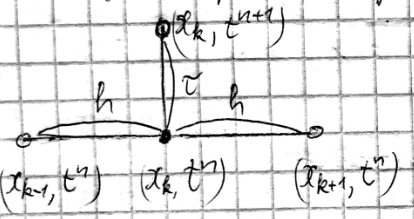
\includegraphics[width = 0.8\linewidth]{img_411}\\
\begin{gather}
\frac{u_{k}^{n+1} - u_{k}^{n}}{\tau} + a \frac{u_{k+1}^{n} - u_{k-1}^{n}}{2h} - D \frac{u_{k+1}^{n} - 2u_{k}^{n} + u_{k-1}^{n}}{h^2} = 0;\\
\nu = \frac{\tau}{2h}; \text\ae = \frac{\tau}{h^2}.\\
u_{k}^{n+1} = \underbrace{(D \text\ae + a \nu)}_{=0} u_{k-1}^{n} + \underbrace{(1-2D \text\ae)}_{\geq 0} u_{k}^{n} + \underbrace{(D \text\ae - a \nu)}_{\geq 0} u_{k+1}^{n}\\
|a|\nu \leq D \text\ae \Longleftrightarrow |a|\frac{\cancel{\tau}}{2 \cancel{h}} \leq \frac{\cancel{\tau}}{h^{\cancel{2}}}\\
\begin{cases}
|a|h \leq 2D \\
2D \text\ae \leq 1 \Longleftrightarrow \frac{2D \tau}{h^2} \leq 1
\end{cases}
\end{gather}
\end{document}
